\subsection{Numerical Approximation and Analysis}\label{sec:set-algorithm}
We present a non-intrusive algorithm based on Monte-Carlo sampling\---initially introduced in \cite{BET+14} and further analyzed in \cite{BET+14-arxiv}\---that is structured in four stages (written as four independent for-loops) that are linked to the stages in Fig.~\ref{fig:scheme}.
We direct the interested reader to \cite{BET+14-arxiv} for more detailed information and analysis of this algorithm, e.g., on the requirement of a sampler being ``$\pborel$-consistent'' to ensure convergence.


\begin{algorithm}[hbtp]
\DontPrintSemicolon
Choose a discretization partition $\set{D_\idisc}_{\idisc=1}^{\ndiscs}$ of $\dspace$.\\
	\For{$\idisc = 1, \hdots, \ndiscs$}{
			Compute $p_{\dspace, \idisc} = \dataP(D_\idisc)$.
	}
	Choose samples $\set{\param^{(\iparam)}}_{\iparam=1}^{\nsamps} \subset \pspace$, which implicitly defines a Voronoi-cell partition $\set{\VV_\iparam}_{\iparam=1}^{\nsamps}$ of $\pspace$.\\
	\For{$\iparam = 1, \hdots, \nsamps$}{
	Compute $\qoi_\iparam = \qoi(\param^{(\iparam)})$.\\
	Let $\OO_\idisc = \set{\iparam: \qoi_\iparam \in D_\idisc}$.\\
	Compute approximations $V_\iparam \approx \pmeas (\VV_\iparam)$.
	}
	\For{$\idisc = 1, \hdots, \ndiscs$}{
	Compute $\CC_\idisc = \set{\iparam:Q_\iparam \in D_\idisc}$.
	}
	\For{$\iparam = 1, \hdots, \nsamps$}{
	Compute $p_{\pspace, \iparam} = \left ( V_\iparam / \sum_{j\in \CC_{\OO_\iparam} } V_j \right ) p_{\dspace, \OO_\iparam}$.
	}
	For any $A\in \pborel$, compute
	\begin{equation}
	\PP_{\pspace, \ndiscs, \nsamps} (A) = \sum_{\iparam=1}^\nsamps p_{\pspace, \iparam} \Chi_{\VV_\iparam} (A)
	\end{equation}
 \caption{Numerical Approximation of the Inverse Density}
 \label{alg:inv_density}
\end{algorithm}


The first two stages correspond to formulating the discretized version of the SIP given in step (S1) in Fig.~\ref{fig:scheme}.
We first discretize the probability space $\Ospace$.
Then, we simultaneously discretize the measure space $(\pspace, \pborel, \pmeas)$ and construct a simple-function approximation to the map $\qoi$.
These stages introduce the primary sources of error, and the third and fourth stages may be thought of as solving the discretized SIP exactly.
The samples that are used to describe $\pspace$ implicitly define a set of Voronoi cells $\set{\VV_\iparam}_{\iparam=1}^{\nsamps}$, which can be seen in Figure~\ref{fig:voronoi_cells}.
Each sample set defines a fundamentally different geometry.

\begin{figure}[ht]
\centering
	\begin{minipage}{.475\textwidth}
		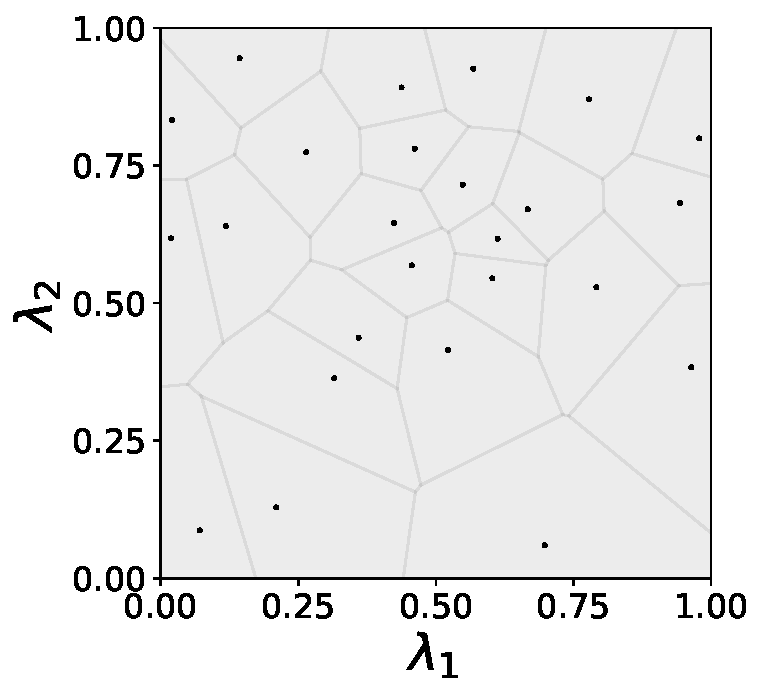
\includegraphics[width=\linewidth]{./images/voronoi_diagrams/voronoi_diagram_N25_r0}
	\end{minipage}
\caption{
Voronoi-cell discretization (partition) induced by $\nsamps = 25 $ uniform i.i.d.~random samples in $\pspace = [0,1]^2$.
}
\label{fig:voronoi_cells}
\end{figure}

The third stage then identifies the collection of Voronoi cells in $\pspace$ that approximate the contour events in $\cborel$ defined by $\qoi^{-1}(D_\idisc)$ for $\idisc=1,\hdots,\ndiscs$. This allows us to formulate the consistent solution to the discretized SIP on $(\pspace, \cborel, \contourP)$ as illustrated in step (S2) of Fig.~\ref{fig:scheme}.
Finally, the fourth stage\---associated with step (S3) in Fig.~\ref{fig:scheme}\---uses a discrete version of the ansatz to approximate the probability of $\VV_\iparam$ for $\iparam=1,\dots,\nsamps$.
This results in an approximate probability measure, denoted by $\PP_{\pspace, \ndiscs, \nsamps}$, which produces the same probability estimates for events $A$ and $A\setminus \set{ \param^{(\iparam)} }_{\iparam=1}^\nsamps$, which are identical almost everywhere with respect to $\pmeas$.

Note that Algorithm~\ref{alg:inv_density} makes no mention of the method by which the samples $\set{ \param^{(\iparam)} }_{\iparam=1}^{\nsamps}$ were generated or sets in $\set{D_\idisc}_{\idisc=1}^{\ndiscs}$ are chosen.
$\set{ \param^{(\iparam)} }_{\iparam=1}^{\nsamps}$ may be generated using uniform random sampling, latin hypercube sampling, or even regular grids.
A thorough discussion of the choices involved in making such decisions is beyond the scope of this work, though we touch briefly on the discretization of $\dspace$ below.
